\documentclass[12pt,a4paper,titlepage,final]{article}
\usepackage[czech]{babel}
\usepackage[utf8]{inputenc}
\usepackage[bookmarksopen,colorlinks,plainpages=false,urlcolor=blue,unicode]{hyperref}
\usepackage{url}
\usepackage{float}
\usepackage{ifthen}
\usepackage[dvipdf]{graphicx}
\usepackage[top=3.5cm, left=2.5cm, text={17cm, 24cm}, ignorefoot]{geometry}

\begin{document}
\newpage

%%%%%%%%%%%%%%%%%%%%%%%%%%%%%%%%%%%%%%%%%%%%%%%%%%%%%%%%%%%%%%%%%%%%%%%%%%%%%%
% titulní strana
\def\name{Lukáš Vokráčko}
\def\login{xvokra00}
\def\subject{Paralelní a distribuované algoritmy}
\def\project{Carry Look Ahead Parallel Binary Adder}

\newboolean{frontpage}
% \setboolean{frontpage}{true}
\setboolean{frontpage}{false}

\ifthenelse{\boolean{frontpage}}
{
	\pagestyle{empty}
	\input{title.tex}
	\tableofcontents
	\newpage
	\pagestyle{plain}
}
{
	\pagestyle{plain}
	% \vspace*{2px}
	\hfill \name, \login \\
	\vspace*{5px}
	{\LARGE \subject}  \\
	{\LARGE \project}  \\
}

\pagenumbering{arabic}
\setcounter{page}{1}
%%%%%%%%%%%%%%%%%%%%%%%%%%%%%%%%%%%%%%%%%%%%%%%%%%%%%%%%%%%%%%%%%%%%%%%%%%%%%%

\section{Analýza algoritmu}
Algoritmus \texttt{Carry look ahead parallel binary adder} je založen na algoritmu \texttt{scan} a speciální operaci, 
která slouží pro výpočet carry. Algoritmus \texttt{scan} pro $n$ položek (listových uzlů) je vypočítán pomocí 
binárního stromu, do kterého jsou uspořádány procesory, jehož výška je $log_{2}{n}+1$. Pro výpočet carry a jeho zpětnou propagaci 
do listových uzlů jsou nutné dva průchody tímto stromem, z čehož vychází časová složitost $t(n) = O(log_{2}{n})$ a prostorová složitost $p(n) = O(n)$,
neboť každý uzel stromu odpovídá jednomu procesoru, přesně tedy $2*n-1$ procesorů.
Z toho vychází celková cena $c(n) = O(n*log_{2}{n})$. V této implementaci není využita celá operace \texttt{scan}, ale pouze její část, \texttt{prescan},
která je pro výpočet dostatečná, neboť hodnotu, která by byla získána rozšířením na operaci \texttt{scan} lze získat již v kořenovém uzlu. Toto zjednodušení
nemá vliv na třídu časové složitosti, protože rozšířením na plnohodnotnou operaci \texttt{scan} by došlo k přidání posunutí, které má konstantní složitost, a 
dalšímu průchodu stromu s logaritmickou složitostí.

\section{Implementace}
Program je implementován v jazyce C++ s využití knihovny \url{https://www.open-mpi.org/}.
Pro spuštění je vytvořen skript \texttt{test}, který přeloží program \texttt{clapba} a spustí ho v prostředí \texttt{MPI}. 
Výstupem programu jsou dvojice ve tvaru \texttt{id procesoru:bit}. Volitelně se na výstupu může objevit řádek obsahující text \texttt{overflow}
pokud dojde k přenosu z významově nejvyššího bitu (\texttt{MSB}).

\section{Experimenty}
Experimenty s implementovaným algoritmem byly prováděny se vstupy dvou binárních čísel stejné délky, která vždy odpovídala $2^n$ pro $ n = 1, 2, .., 64$.
Experiment pro každou délku byl proveden v deseti iteracích a zde prezentované výsledky jsou aritmetickým průměrem naměřených hodnot, čímž 
byl zmenšen vliv okolí. Experimenty byly spouštěny na jednoprocesorovém systému, což způsobilo, že \texttt{MPI} simulovalo procesory vytvářením nových procesů,
které poté běžely sekvenčně. V následujícím grafu jsou zaneseny naměřené hodnoty. \\ 
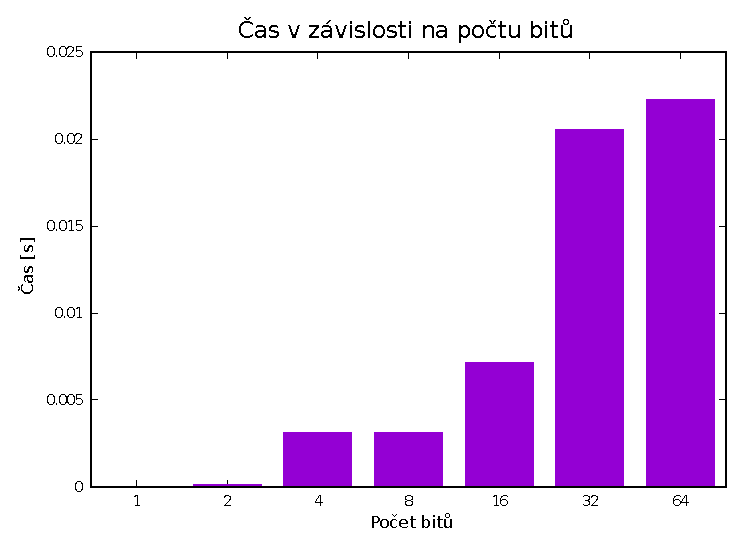
\includegraphics[width=14cm,keepaspectratio]{time.eps}

\section{Komunikační protokol}
Na počátku zašle kořenový uzel odpovídající dvojici bitů všem listovým procesorům, 
poté každý uzel vyjma kořene odesílá a přijímá svoji hodnotu od přímého rodičovského uzlu.

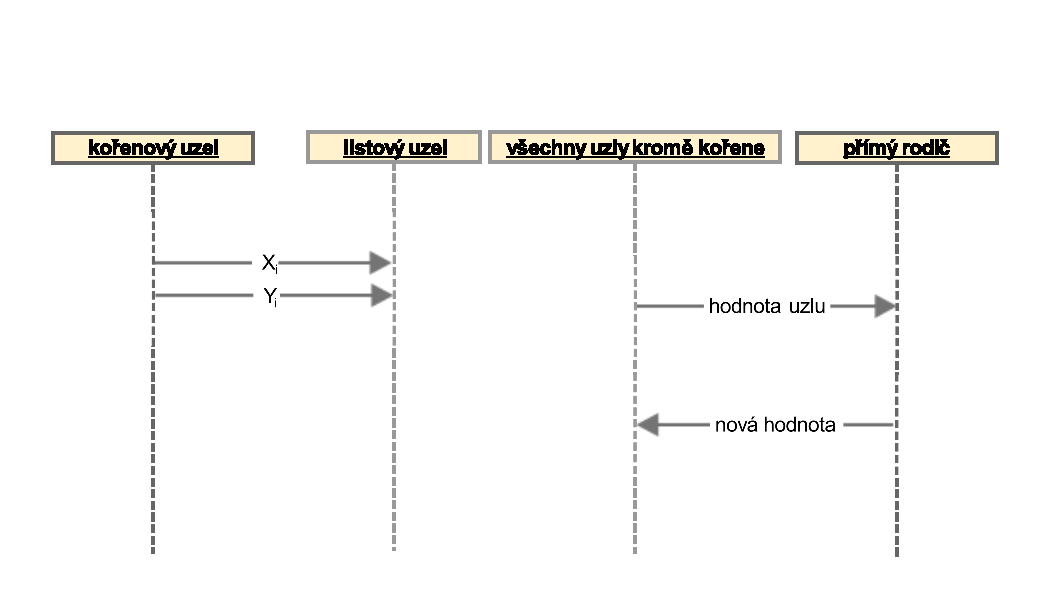
\includegraphics[width=14cm,keepaspectratio]{sequence.eps}

\section{Závěr}
Naměřené hodnoty při experimentování neodpovídají třídě časové složitosti $t(n) = O(log_{2}{n})$, neboť byly prováděny na jednoprocesorovém stroji a tudíž by naměřené hodnoty měly odpovídat celkové ceně algoritmu $c(t) = O(n*log_{2}{n})$, neboť všechny procesy jsou vykonávány sekvenčně, čemuž také
přibližně odpovídají výsledky získané experimenty.
\end{document}
